% include data sheets/links to things that we bought or would like to buy in the future to further improve this project.

\begin{centering}
% Edit me. I'm preformatted
\begin{table}[!ht]\hspace{-2cm}


\centering

\resizebox{1\textwidth}{!}{\begin{tabular}{|c|c|c|c|c|}

\hline
Item Description & Price & Quantity & Subtotal & Supplier\\
\hline
Raspberry Pi 3 Starter Kit & \$50 & 4 & \$200 & Amazon\\
\hline
Raspberry Pi 3 Complete Camera Kit & \$90 & 1 & \$90 & Amazon\\
\hline
Raspberry Pi 0 Wireless Starter Kit & \$23 & 5 & \$115 & Amazon\\
\hline
Hardware mounting components (screws,nuts,bolts) & \$50 & 1 & \$10 & ACE\\
\hline
NeoPixel Ring & \$15 & 4 & \$60 & Amazon\\
\hline
Ping Sensor (HC-SR04) (Pack of 5) & \$10 & 1 & \$10 & Amazon\\
\hline
Magnetometer Sensor & \$3.50 & 5 & \$18 & Amazon\\
\hline
MicroUSB 10 pack & \$4.50 & 1 & \$5 & Amazon\\
\hline
SanDisk 8 GB SD Card & \$6 & 5 & \$30 & Amazon\\
\hline
Acrylic Tube  & \$90 & 3 & \$270 & Taps Plastic\\
\hline
\textbf{Total} & & & \textbf{\$808} &\\
\hline

\end{tabular}}
\end{table}
\end{centering}
\vspace{0.1cm}


\begin{figure}[ht]
  \caption{Pinout of the Raspberry pi 3}
  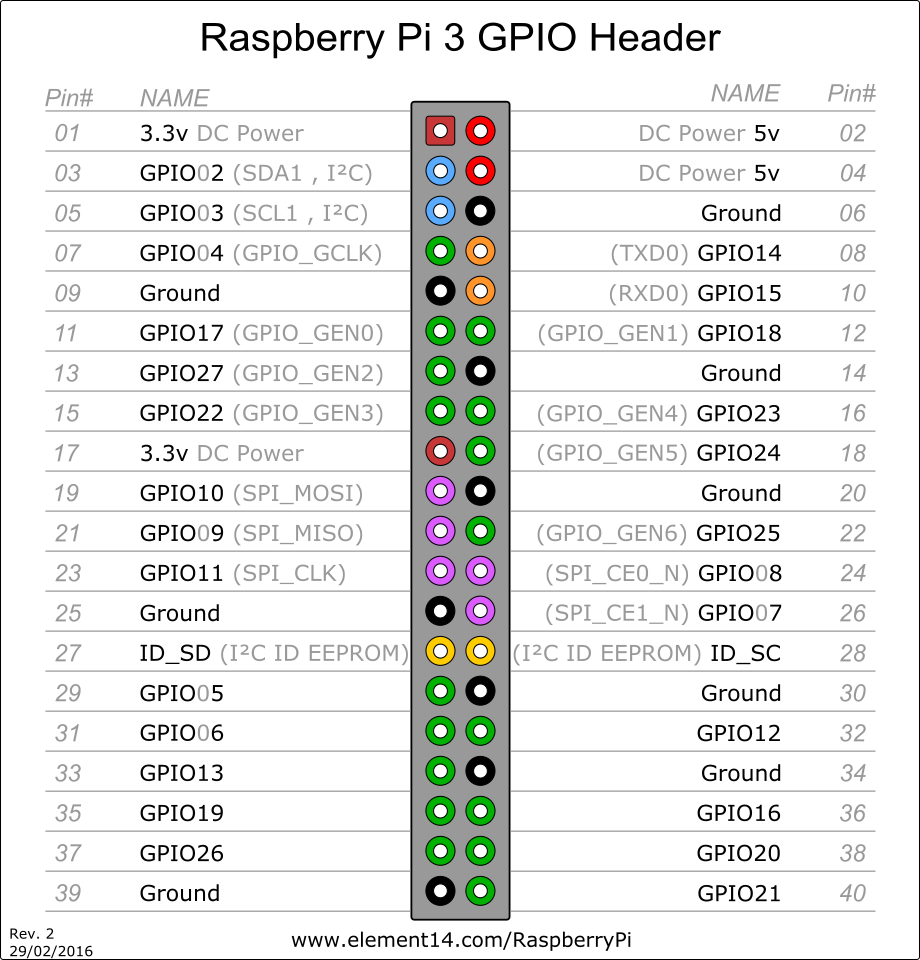
\includegraphics[width=0.7\textwidth]{pictures/pi3_gpio.png}
  \label{fig:rpi}
\end{figure}


\begin{figure}[ht]
  \caption{Pinout of the arduino nano}
  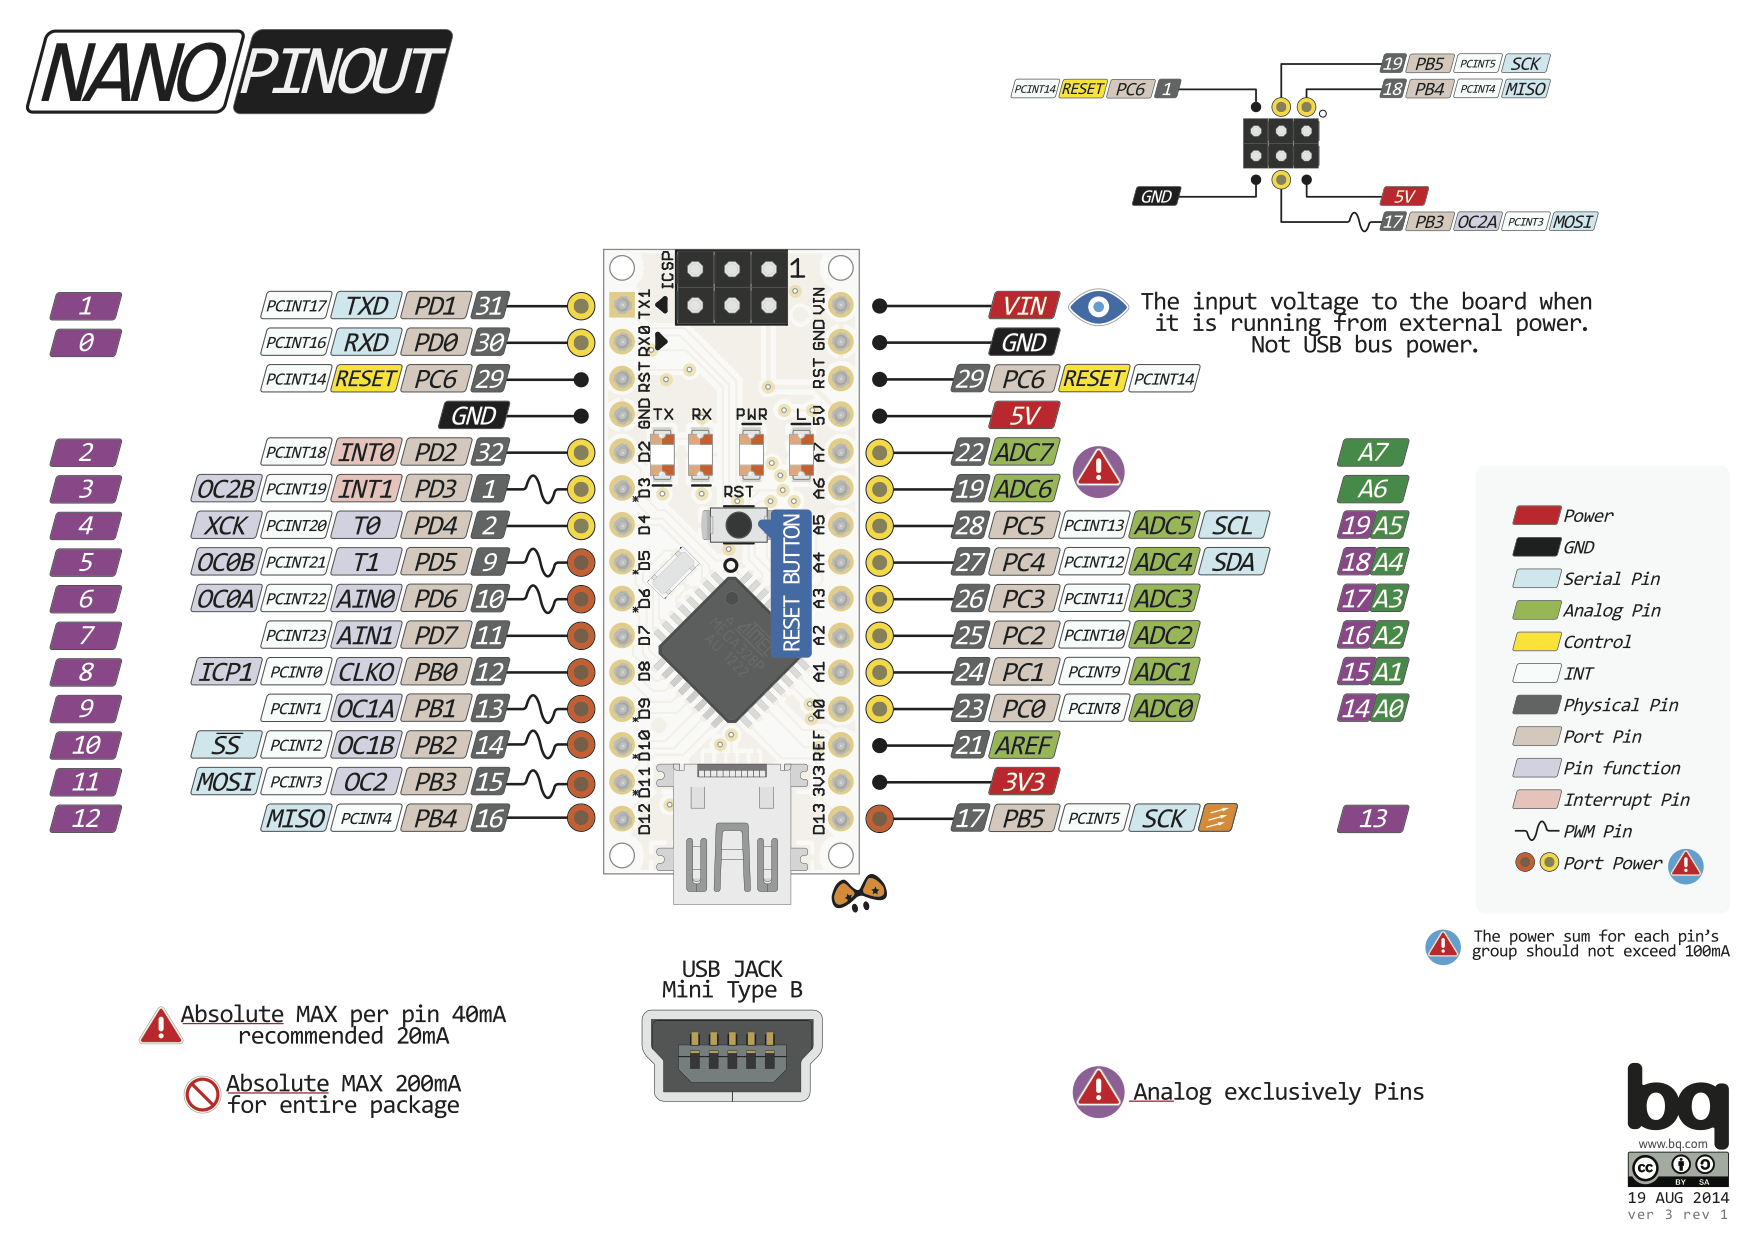
\includegraphics[width=1\textwidth]{pictures/nano.png}
\end{figure}
